\documentclass[]{article}

\usepackage[utf8]{inputenc}
\usepackage[english]{babel}
\usepackage{graphicx}
\usepackage{url}
%opening
\title{Übung 1 // DOC}
\author{Benjamin Blackmann, Aryan Carlos Rezai, Valentin Risch}

\begin{document}

\maketitle


\textbf{1.1 }Als UI Bibliothek für die Benutzeroberfläche haben wir uns für JavaFX entschieden. Für die Implementierung der ersten Aufgabe haben wir auf eine Controller Klasse verzichtet da das Programm zu rudimentär ist um diesen Aufwand zu betreiben. 
Um ein BufferedImage in JavaFX zu verwenden haben wir hier auf die Methode toFXImage() der SwingFXUtils Klasse zurück gegriffen.\\

\textbf{1.2 }Für die zweite Aufgabe hingegen wird pixelweise der Farbwert des Image Objektes ausgelesen und in ein WritableImage, welches in JavaFx eine direkte Unterklasse der Image Implementierung ist geschrieben.
Große Schwierigkeiten bereitete uns die Implementierung einer sich in der Größe verändernden View für das Bild. Da man im Controller der Gui keinen Zugriff auf das Stage Objekt hat fügen wir in der initzialize Methode Event Listener für das “width” und “height” attribut des Root Elements hinzu, in unserem Fall eine Anchor Pane. Wird nun die Größe verändert wird die initImageView() Methode neu angestoßen.\\

\textbf{1.3    Vektoren und Matrizen Bibliothek}\\

\begin{center}
	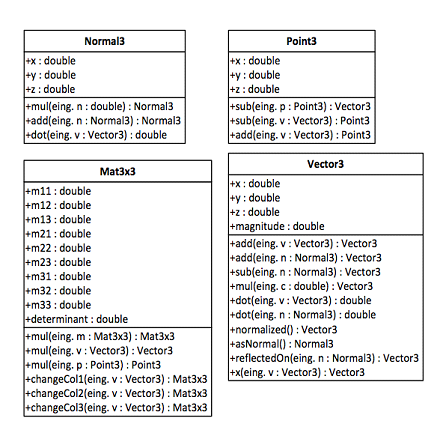
\includegraphics[scale=1]{01.png}\\
\end{center}

Die Implementierung der Vektoren und Matrizen Bibliothek verlief mithilfe der Klassendiagramme größtenteils problemlos.
Alle 4 Klassen - Point3 / Normal3 / Vector3 / Mat3x3 wurden immutable implementiert, zusätzlich wurde eine TestSuite mit JUnit4 erstellt.\\

\textbf{1.3.1 Implementierung}\\

Anfangs gab es Probleme beim finden der richtigen Formel für die Reflexion von Vektoren, da es unterschiedliche Möglichkeiten gibt, diese durchzuführen. 
Wir entschieden uns für jene, die es durch Vektoren Projektion ermöglicht, den reflektierten Vektor zu berechnen.
Mathematische Formel:
\[ r = d - 2 (d*n)^n\] 
(wobei: 
r :    resultierender, “Reflexion-Vektor” (Projektion)
d :    der gegebene Vektor, der reflektiert werden soll
n :    der Normalenvektor der Ebene, an der  d  reflektiert werden soll)\\
Anschließend muss die Richtung des projizierten Vektors  r  noch negiert werden (-1).
Damit erschließt sich folgende Methode in unserem Code:\\

\begin{center}
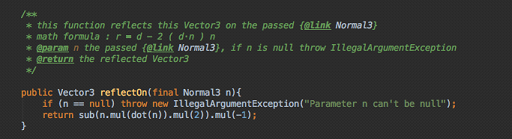
\includegraphics[scale=1]{02.png}\\
\end{center}


Nachdem alle Methoden implementiert waren, wurden noch die letzten Warnungen im Code behoben. Für die Fields der Klassen wurde hier der Ausdruck 
@SuppressWarnings("WeakerAccess")
benutzt.\\

\begin{center}
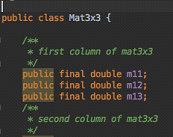
\includegraphics[scale=1]{03.png}
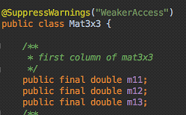
\includegraphics[scale=1]{04.png}\\  
\end{center}


\textbf{1.3.2 TestSuite}\\

Das Implementieren der TestSuite verlief größtenteils problemlos.
Als erstes wurde mithilfe von IntelliJ ein Testgerüst für jede Klasse erstellt, und anschließend wurden alle zu testenden Methoden mit den richtigen Werten getestet.
Hierbei kam es bei den Methoden reflectOn() und x() der Klasse Vector3 zu Komplikationen mit den resultierenden Testwerten.\\

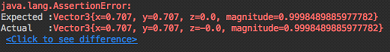
\includegraphics[scale=1]{05.png}\\

Leider konnten wir diesen Fehler bis jetzt nicht beheben, die Suche ergab bisher z.B. folgendes: \url{http://dev.clojure.org/jira/browse/CLJ-1860 }
Die Werte 0.0 und -0.0 ergeben unter .equals() true, jedoch beinhalten sie einen unterschiedlichen Hash-Wert. 
Das Problem wurde temporär gefixt, in dem die resultierenden Werte des Vektors in -0.0 geändert wurden.






\end{document}
